% ============================================================
%  BRUTALIST THESIS POSTER — A1 Portrait
%  FIXED: Title tracking, title rules, and complementarity alignment
% ============================================================

\documentclass{article}

% ── Core packages ───────────────────────────────────────────
\usepackage[a1paper, portrait,
            top=1.0cm, bottom=1.0cm,
            left=1.2cm, right=1.2cm]{geometry}
\pagestyle{empty}

\usepackage{fontspec}
\usepackage{microtype}           % REQUIRED for \textls letter-spacing
\usepackage{xcolor}
\usepackage{graphicx}
\usepackage{booktabs}
\usepackage{array}
\usepackage{colortbl}
\usepackage{amsmath}
\usepackage{adjustbox}
\usepackage[most]{tcolorbox}
\usepackage{dashrule}            % \hdashrule
\usepackage{calc}

% ── Global base font size (A1 needs ~20pt body) ─────────────
\makeatletter
\renewcommand\normalsize{%
  \@setfontsize\normalsize{18pt}{23pt}%
  \abovedisplayskip 10pt
  \belowdisplayskip 10pt}
\renewcommand\large{\@setfontsize\large{21pt}{26pt}}
\renewcommand\Large{\@setfontsize\Large{24pt}{30pt}}
\renewcommand\huge{\@setfontsize\huge{34pt}{40pt}}
\makeatother
\normalsize

% ── Fonts ───────────────────────────────────────────────────
\newfontfamily\archivo{ArchivoBlack}[
  Path        = fonts/,
  Extension   = .ttf,
  UprightFont = *-Regular
]

\setmainfont{SourceSansPro}[
  Path           = fonts/,
  Extension      = .ttf,
  UprightFont    = *-Regular,
  BoldFont       = *-Bold,
  ItalicFont     = *-Italic,
  BoldItalicFont = *-BoldItalic
]

\newfontfamily\mono{JetBrainsMono}[
  Path           = fonts/,
  Extension      = .ttf,
  UprightFont    = *-Regular,
  BoldFont       = *-Bold,
  ItalicFont     = *-Italic,
  BoldItalicFont = *-BoldItalic
]

% ── Colour palette ──────────────────────────────────────────
\definecolor{Navy}{HTML}{0D1F5C}
\definecolor{NavyMid}{HTML}{1A3380}
\definecolor{Orange}{HTML}{FF8C00}
\definecolor{AccentBlue}{HTML}{4A6FD4}
\definecolor{AccentLight}{HTML}{99B0FF}
\definecolor{PaperBg}{HTML}{F0EDE6}
\definecolor{BoxBg}{HTML}{FAF8F2}
\definecolor{TableStripe}{HTML}{EDE9DF}
\definecolor{TextDark}{HTML}{111111}
\definecolor{TextMid}{HTML}{444444}
\definecolor{GreenHL}{HTML}{0A6640}

\pagecolor{PaperBg}
\color{TextDark}
\setlength{\parindent}{0pt}
\setlength{\parskip}{0.3em}

% ── Highlight macros ────────────────────────────────────────
\newcommand{\hlorg}[1]{%
  \colorbox{Orange}{\color{white}\mono\fontsize{17}{19}\selectfont\textbf{#1}}%
}
\newcommand{\hlnavy}[1]{%
  \colorbox{Navy}{\color{white}\mono\fontsize{17}{19}\selectfont\textbf{#1}}%
}
\newcommand{\hlgreen}[1]{%
  \colorbox{GreenHL}{\color{white}\mono\fontsize{17}{19}\selectfont\textbf{#1}}%
}

% ── Pipeline step macro ─────────────────────────────────────
\newcommand{\pipestep}[1]{%
  \colorbox{Navy}{\color{white}\mono\fontsize{16}{18}\selectfont\textbf{\ #1\ }}%
}
\newcommand{\pipearrow}{%
  {\color{Orange}\bfseries\fontsize{22}{24}\selectfont\ \textrightarrow\ }%
}

% ── BRUTALIST BOX ───────────────────────────────────────────
\newtcolorbox{brutebox}[1]{
  enhanced,
  colback=BoxBg,
  colframe=TextDark,
  boxrule=2.5pt,
  arc=0pt,
  outer arc=0pt,
  colbacktitle=Navy,
  coltitle=white,
  fonttitle=\mono\fontsize{22}{26}\selectfont\bfseries,
  attach boxed title to top left={xshift=0pt, yshift=0pt},
  boxed title style={
    colback=Navy,
    colframe=Navy,
    arc=0pt,
    outer arc=0pt,
    boxrule=0pt,
    left=0pt, right=0pt,
    top=8pt, bottom=8pt,
    width=\linewidth+5pt,
    enlarge left by=-2.5pt,
  },
  title={%
    \centering
    \hdashrule[0.6ex]{1cm}{1pt}{3pt 3pt}\quad
    \textls[110]{#1}%
    \quad\hdashrule[0.6ex]{1cm}{1pt}{3pt 3pt}%
  },
  top=0.4cm,
  bottom=0.4cm,
  left=0.8cm,
  right=0.8cm,
  fontupper=\normalsize,
  before upper={\vspace{0.1em}}
}

% ── Bullet list inside boxes ─────────────────────────────────
\newenvironment{brutelist}{%
  \begin{list}{{\color{Orange}\bfseries\fontsize{22}{24}\selectfont->}}{%
    \setlength{\leftmargin}{1.8em}%
    \setlength{\itemsep}{0.15em}%
    \setlength{\parsep}{0pt}%
    \normalsize
  }%
}{%
  \end{list}%
}

% ── Centred column type ──────────────────────────────────────
\newcolumntype{M}[1]{>{\centering\arraybackslash}m{#1}}

% ============================================================
\begin{document}

% Force page limits to expand so everything stays strictly on Page 1
\enlargethispage{30cm}

% ╔══════════════════════════════════════════════════════════╗
% ║                      BANNER                              ║
% ╚══════════════════════════════════════════════════════════╝
\begin{tcolorbox}[
    enhanced,
    colback=Navy,
    colframe=TextDark,
    arc=0pt, outer arc=0pt,
    boxrule=3pt,
    left=1.2cm, right=1.2cm,
    top=0.5cm, bottom=0.5cm
]
  \begin{minipage}[c]{0.09\linewidth}
    \centering
    
\includegraphics[width=\linewidth]{Logo_BK.png}
  \end{minipage}%
  \hfill
  \begin{minipage}[c]{0.48\linewidth}
    \raggedright
    {\mono\fontsize{16}{19}\selectfont\bfseries\color{AccentLight}%
      HO CHI MINH CITY UNIVERSITY OF TECHNOLOGY (HCMUT)}\par
    \vspace{0.12cm}
    {\mono\fontsize{13}{16}\selectfont\color{AccentBlue}%
      FACULTY OF COMPUTER SCIENCE AND ENGINEERING}\par
    \vspace{0.2cm}
    \colorbox{NavyMid}{%
      \color{AccentLight}\mono\fontsize{15}{18}\selectfont\bfseries
      \textls[120]{\ * GRADUATION THESIS\ }%
    }\par
    \vspace{0.2cm}
    {\archivo\fontsize{36}{38}\selectfont\color{white}%
      \MakeUppercase{Leveraging Multimedia Data For}}\par
    {\archivo\fontsize{36}{38}\selectfont\color{Orange}%
      \MakeUppercase{Next Best Action}}\par
    {\archivo\fontsize{36}{38}\selectfont\color{white}%
      \MakeUppercase{Recommendation System}}\par
  \end{minipage}%
  \hfill
  \begin{minipage}[c]{0.13\linewidth}
    \centering
    \colorbox{Orange}{%
      \color{white}\mono\fontsize{18}{21}\selectfont\bfseries
      \textls[60]{\ TOPIC NO. 115\ }%
    }\par
    \vspace{0.15cm}
    \begin{tcolorbox}[
        enhanced, colback=Navy, colframe=AccentBlue,
        arc=0pt, boxrule=2pt, dashed,
        width=5.8cm, height=5.8cm,
        valign=center, halign=center,
        left=0pt, right=0pt, top=0pt, bottom=0pt
      ]
      \color{AccentBlue}\mono\fontsize{16}{20}\selectfont
      QR Code\\[0.3em](to be added)
    \end{tcolorbox}
  \end{minipage}%
  \hfill
  \begin{minipage}[c]{0.21\linewidth}
    \raggedright
    {\mono\fontsize{13}{15}\selectfont\color{PaperBg}\textls[120]{SUPERVISOR}}\par
    \vspace{0.15cm}
    {\fontsize{22}{26}\selectfont\bfseries\color{white}PhD. Le Thanh Van}\par
    \vspace{0.15cm}
    {\color{AccentBlue}\hdashrule{\linewidth}{1pt}{3pt 3pt}}\par
    \vspace{0.15cm}
    {\mono\fontsize{13}{15}\selectfont\color{PaperBg}\textls[120]{STUDENTS}}\par
    \vspace{0.10cm}
    {\fontsize{20}{24}\selectfont\bfseries\color{white}Dang Minh Khang}\par
    {\mono\fontsize{14}{17}\selectfont\color{PaperBg}2252287}\par
    \vspace{0.10cm}
    {\fontsize{20}{24}\selectfont\bfseries\color{white}Pham Tran Dang Khoa}\par
    {\mono\fontsize{14}{17}\selectfont\color{PaperBg}2252360}\par
    \vspace{0.10cm}
    {\fontsize{20}{24}\selectfont\bfseries\color{white}Le Ha Nguyen Khanh}\par
    {\mono\fontsize{14}{17}\selectfont\color{PaperBg}2252327}\par
  \end{minipage}
\end{tcolorbox}

\nopagebreak
\vspace{-3pt}
\noindent{\color{TextDark}\rule{\linewidth}{3pt}}
\nopagebreak
\vspace{0.35cm}

% ╔══════════════════════════════════════════════════════════╗
% ║                    MAIN BODY                             ║
% ╚══════════════════════════════════════════════════════════╝

\noindent
\begin{minipage}[t]{0.48\linewidth}%
  \vspace{0pt}
  \begin{brutebox}{INTRODUCTION}
    \begin{brutelist}
      \item \textbf{Context:} Major platforms catalogue millions of books, yet traditional recommenders rely on single modalities. They ignore item semantics and fail to capture \hlorg{sequential intent} (recent user clicks).
      \item \textbf{Problem:} Most open-source encoders perform poorly on Vietnamese queries, and production demands \hlnavy{sub-100 ms} response times.
      \item \textbf{Solution:} A \hlorg{dual-mode multimodal} system unifying behavioral graph embeddings, a sequential transformer, and a multilingual encoder over 3M items.
    \end{brutelist}
  \end{brutebox}

  \vspace{0.3cm}

  \begin{brutebox}{OBJECTIVES}
    \begin{brutelist}
      \item \textbf{Design} a dual-mode pipeline integrating Cleora behavioral graph embeddings with DIF-SASRec sequential transformer.
      \item \textbf{Achieve} measurable improvement in HR@10 and NDCG@10 over the prior baseline on 100,000 held-out users.
      \item \textbf{Enable} multilingual semantic search with significantly improved precision on Vietnamese queries.
      \item \textbf{Optimise} warm-cache end-to-end search latency below 100 ms.
    \end{brutelist}
  \end{brutebox}

  \vspace{0.3cm}

  \begin{brutebox}{METHODOLOGY}
    The system operates in two complementary modes:

    \begin{brutelist}
      \item \textbf{Pipeline A (Passive):} Cleora co-purchase graph embeddings narrow candidates to behaviorally related titles. A BGE-M3 mean-profile vector then re-ranks them.
      \item \textbf{Pipeline B (Sequential):} DIF-SASRec transformer with decoupled content and category attention streams models per-user sequential interest.
      \item \textbf{Active Search:} Vietnamese queries translated via NLLB-200. Text/image embeddings (BGE-M3 + CLIP) fused with RRF over FAISS HNSW.
    \end{brutelist}

    \vspace{0.4em}
    {\mono\fontsize{15}{18}\selectfont\bfseries\color{TextMid}%
      \textls[100]{ACTIVE SEARCH PIPELINE:}}\par
    \vspace{0.2cm}
    \pipestep{Query (VI)}\pipearrow
    \pipestep{NLLB-200}\pipearrow
    \pipestep{BGE-M3+CLIP}\pipearrow
    \pipestep{RRF}\pipearrow
    \pipestep{FAISS HNSW}\par

    \vspace{0.4em}
    {\mono\fontsize{15}{18}\selectfont\bfseries\color{TextMid}%
      \textls[100]{PASSIVE RECOMMENDATION:}}\par
    \vspace{0.2cm}
    \pipestep{User History}\pipearrow
    \pipestep{Cleora Graph}\pipearrow
    \pipestep{DIF-SASRec}\pipearrow
    \pipestep{NBA}\par

    \vspace{0.3cm}
    {\centering
      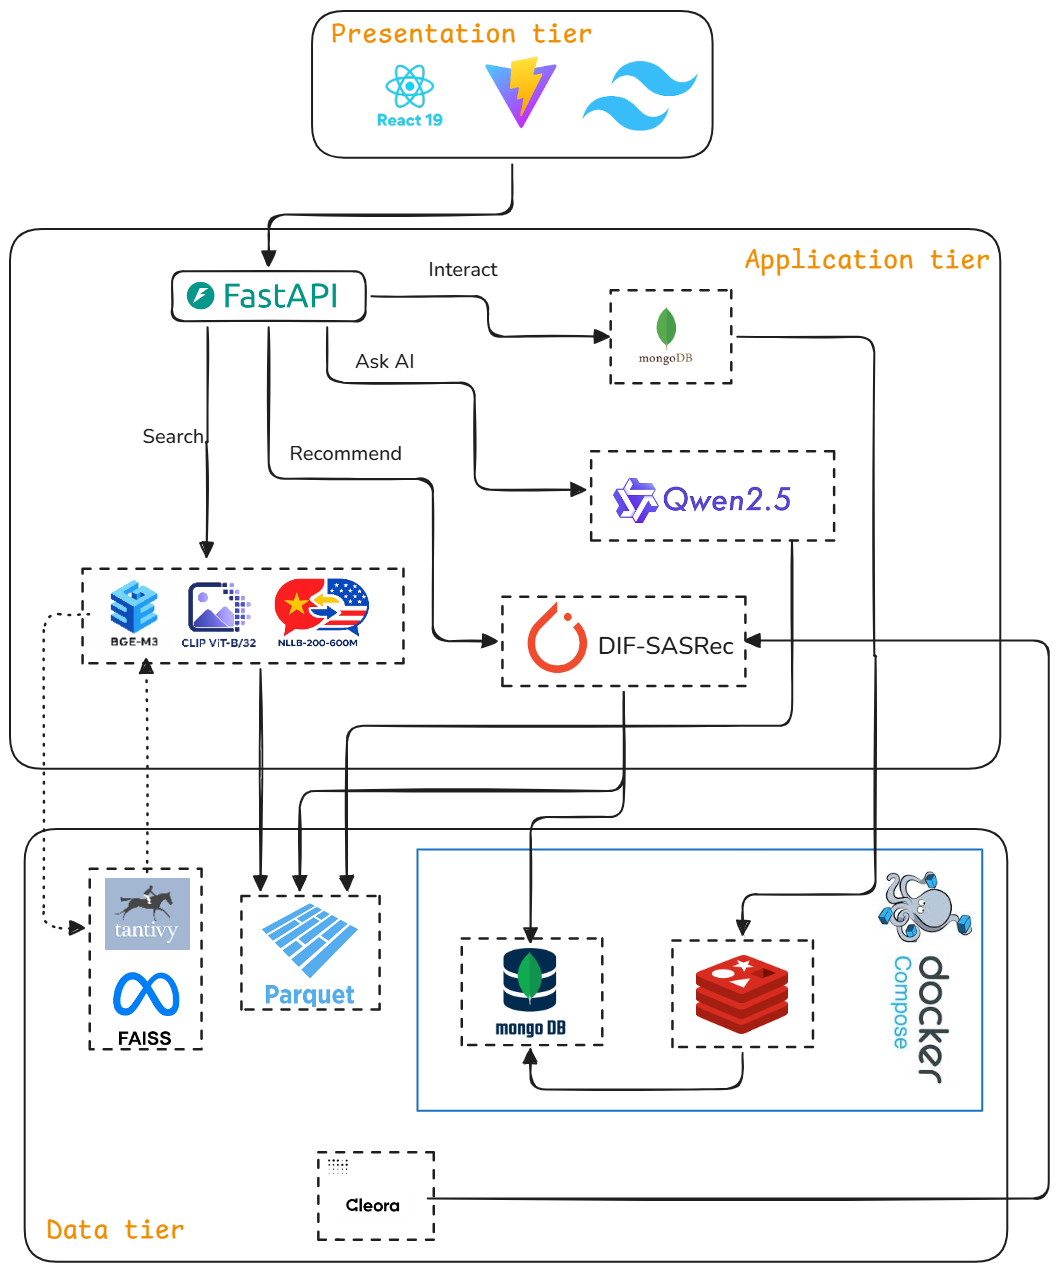
\includegraphics[width=0.80\linewidth]{Fig3.1.png}\par
      \vspace{0.2em}
      {\mono\fontsize{16}{19}\selectfont\color{TextMid}\textit{Figure 1: Overall system architecture.}}\par}
  \end{brutebox}
\end{minipage}%
\hfill
\begin{minipage}[t]{0.49\linewidth}%
  \vspace{0pt}
  \begin{brutebox}{EXPERIMENTS}
    {\mono\fontsize{17}{20}\selectfont\color{TextMid}%
      Dataset: \textbf{Amazon Book Reviews}
      \textbullet\ 100,000 test users \textbullet\ 3.08M items}\par
    \vspace{0.35cm}

    \begin{adjustbox}{width=\linewidth}
    \renewcommand{\arraystretch}{1.4}
    \begin{tabular}{lcccc}
      \toprule
      \rowcolor{Navy}
      {\color{white}\bfseries Method} &
      {\color{AccentLight}\bfseries HR@5} &
      {\color{AccentLight}\bfseries HR@10} &
      {\color{AccentLight}\bfseries NDCG@10} &
      {\color{AccentLight}\bfseries MRR@10} \\
      \midrule
      Random Baseline              & 0.050 & 0.100 & 0.045 & --- \\
      \rowcolor{TableStripe}
      Content Baseline             & 0.360 & 0.435 & 0.302 & 0.261 \\
      GRU-SeqDQN                   & 0.052 & 0.103 & 0.047 & 0.031 \\
      \rowcolor{TableStripe}
      DIF-SASRec (Pipeline B)      & 0.588 & 0.775 & 0.502 & 0.419 \\
      Pipeline A (Cleora+BGE-M3)   & 0.575 & 0.905 & 0.539 & 0.430 \\
      \rowcolor{Navy}
      {\color{white}\bfseries >> System ($A \cup B$)} &
      {\color{AccentLight}---} &
      {\color{Orange}\bfseries 0.974} &
      {\color{Orange}\bfseries 0.557} &
      {\color{AccentLight}---} \\
      \bottomrule
    \end{tabular}
    \end{adjustbox}

    \vspace{0.3cm}
    {\centering
      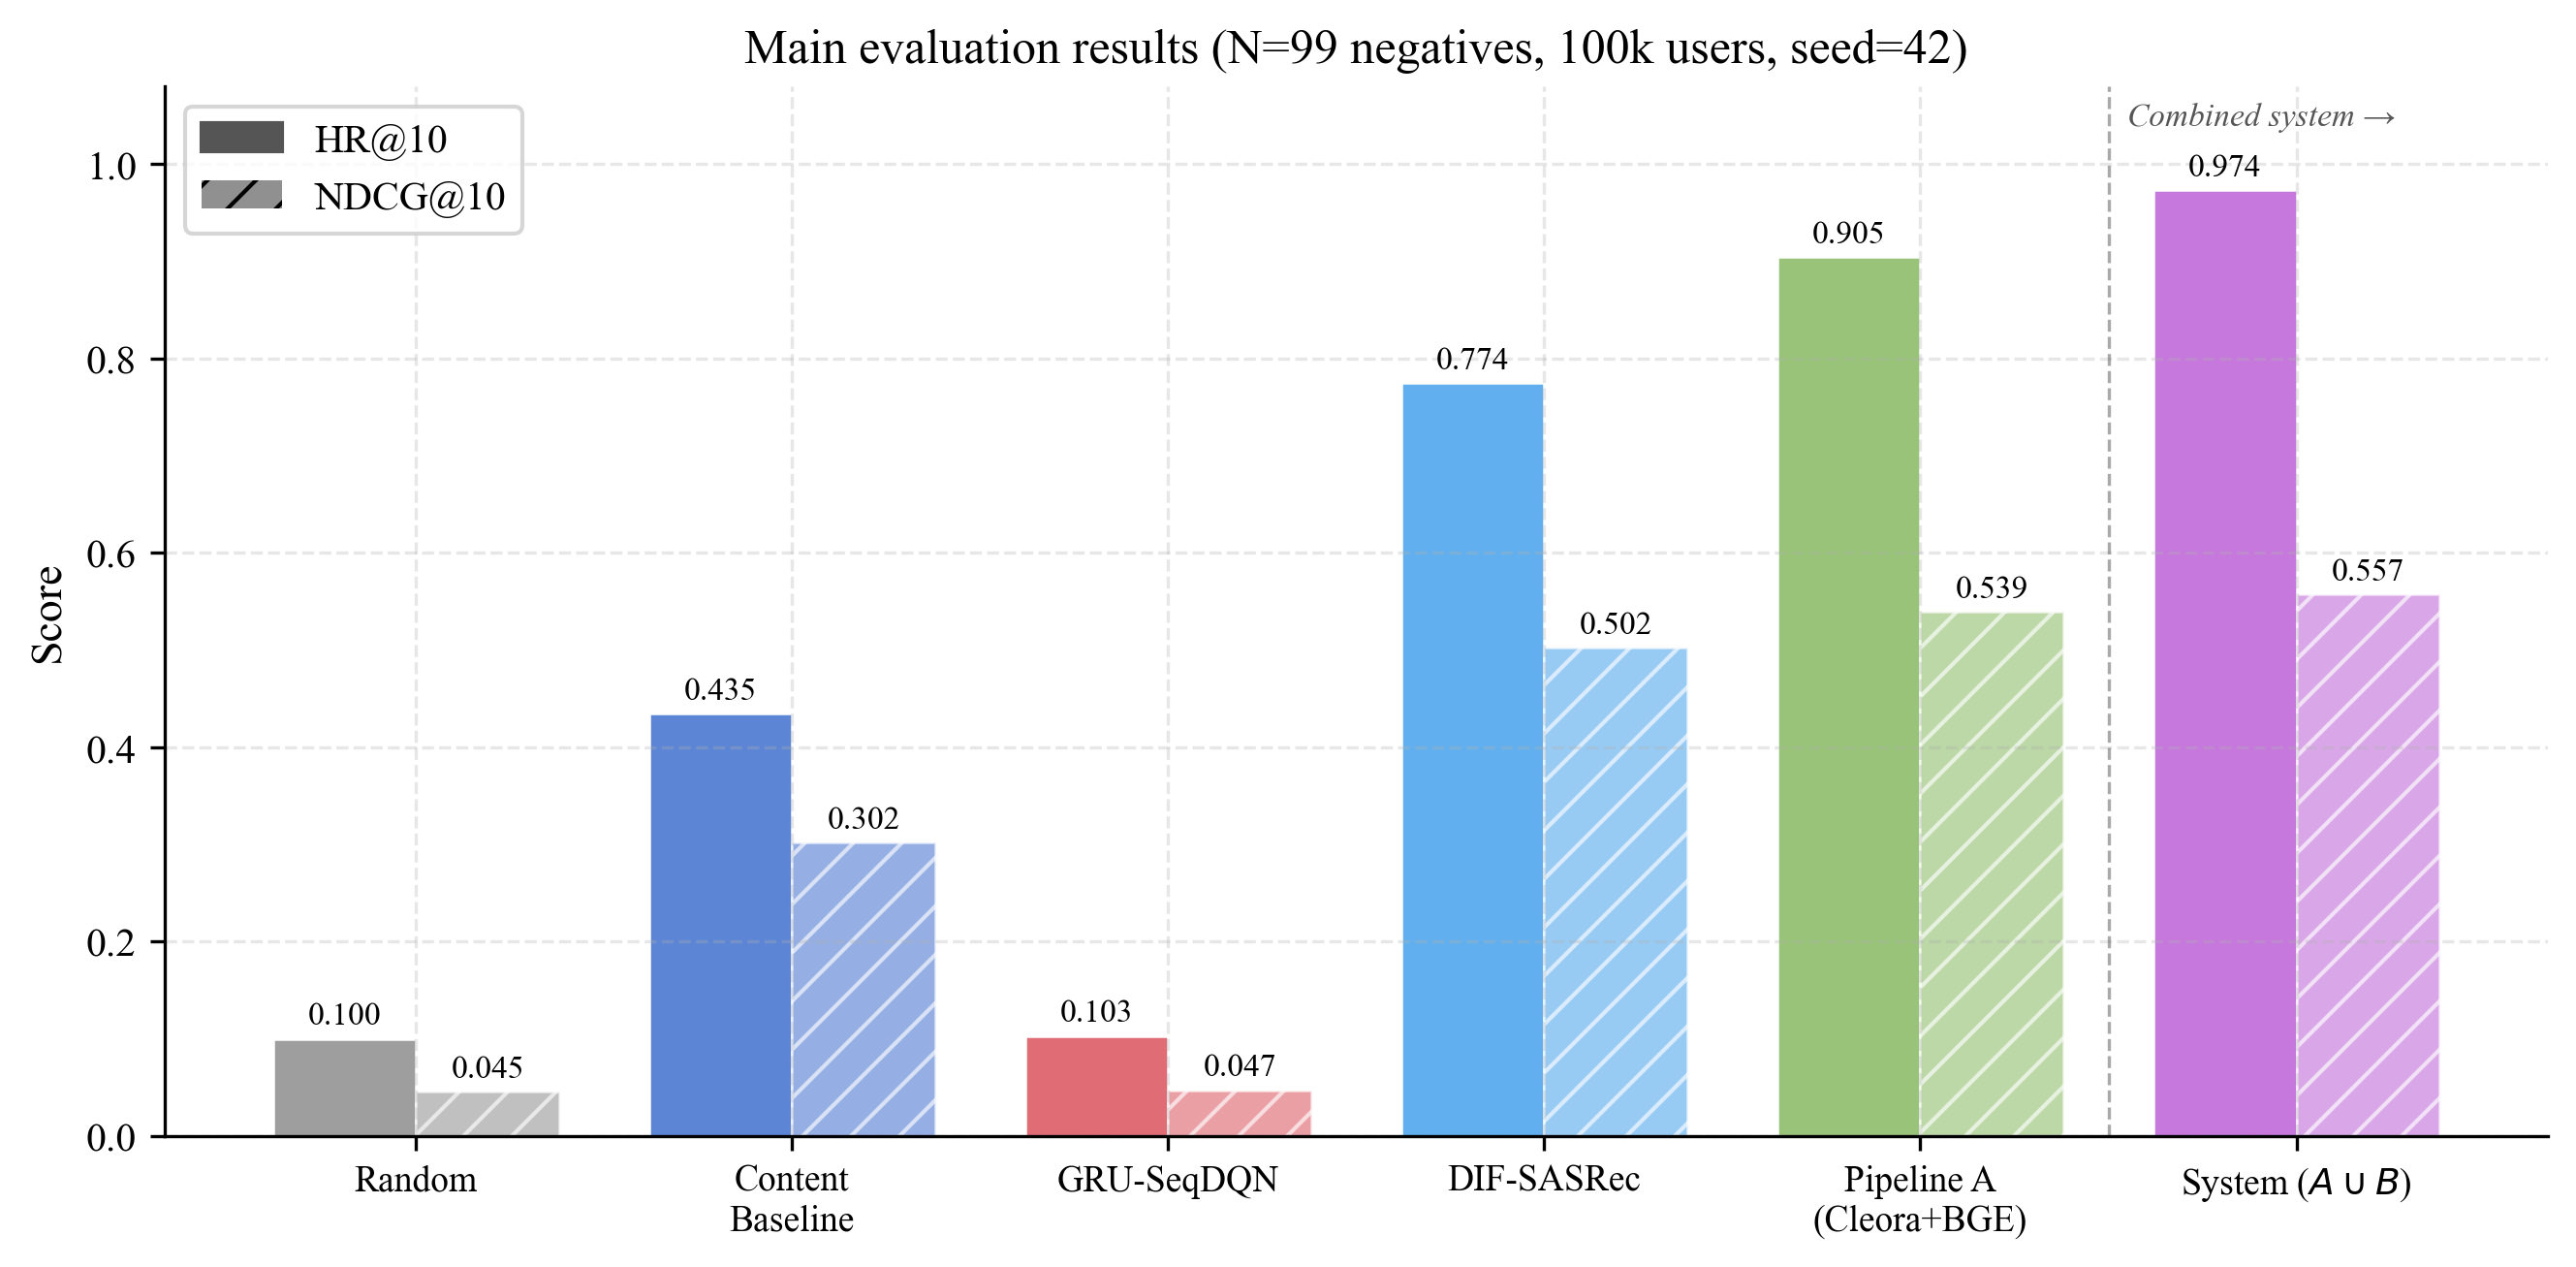
\includegraphics[width=0.80\linewidth]{fig_main_results.png}\par
      \vspace{0.2em}
      {\mono\fontsize{16}{19}\selectfont\color{TextMid}\textit{Figure 2: HR@10 and NDCG@10 across all methods.}}\par}
  \end{brutebox}

  \vspace{0.3cm}

  \begin{brutebox}{WHY THE UNION WINS: PIPELINE COMPLEMENTARITY}
    \begin{minipage}[t]{0.53\linewidth}%
      \vspace{0pt}%
      \centering
      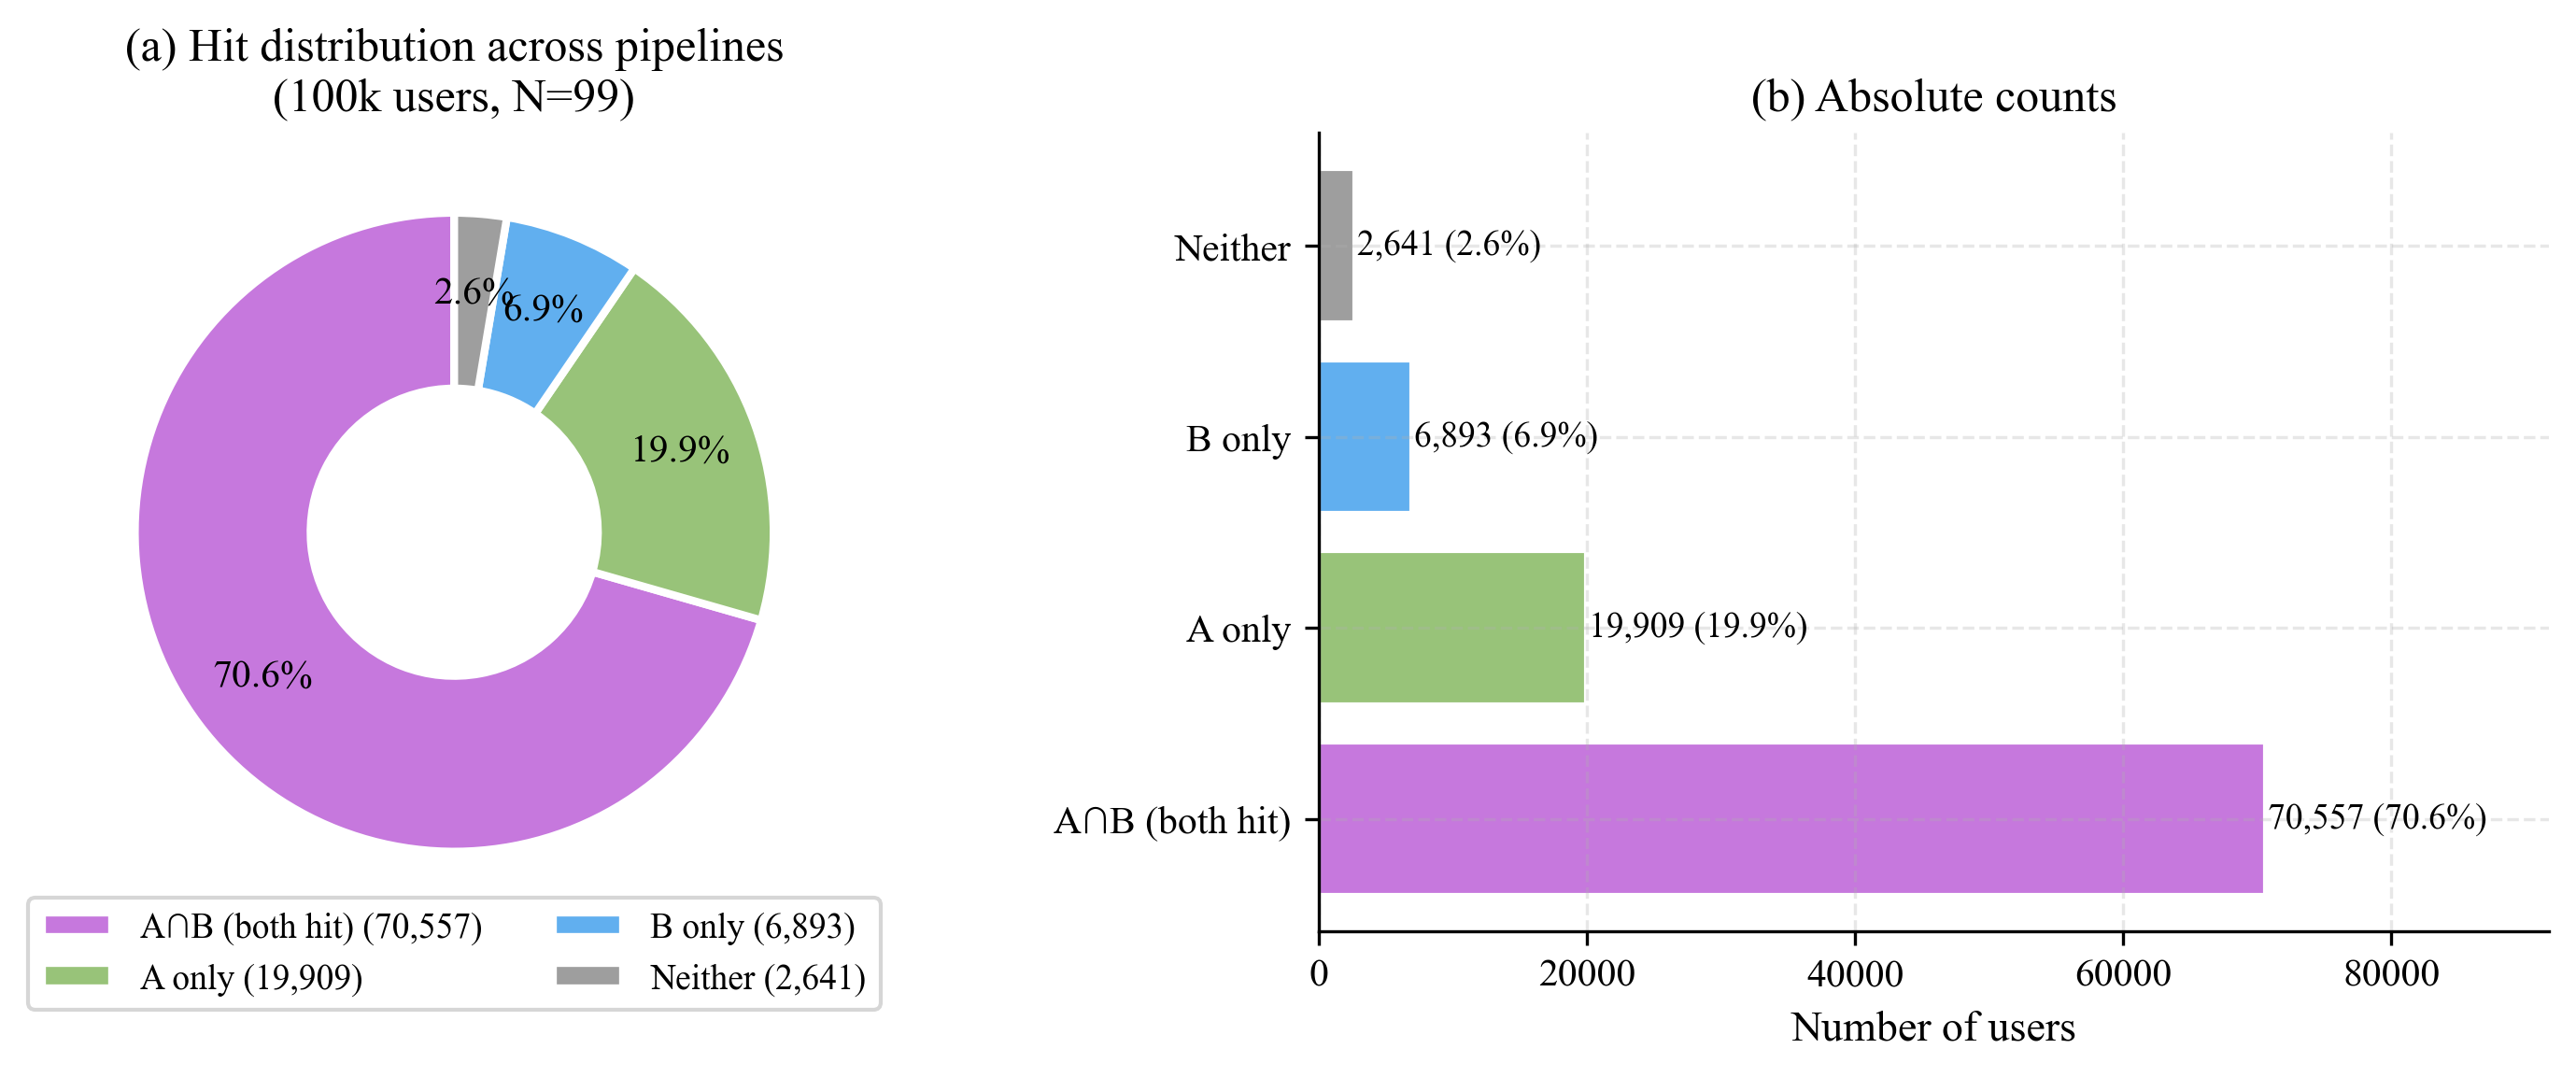
\includegraphics[width=\linewidth]{fig_complementarity.png}\par
      \vspace{0.15em}
      {\mono\fontsize{15}{18}\selectfont\color{TextMid}\textit{Figure 3: Exclusive hits per pipeline (100k users).}}\par
    \end{minipage}%
    \hfill
    \begin{minipage}[t]{0.44\linewidth}%
      \vspace{0pt}%
      \vspace{0.3em}%
      {\fontsize{17}{21}\selectfont
        \textbf{Pipeline A} (Cleora + BGE-M3) retrieves from a \hlorg{behavioral co-purchase graph} — strong for popular and co-bought titles.\par
        \vspace{0.4em}
        \textbf{Pipeline B} (DIF-SASRec) captures \hlnavy{sequential reading intent} — strong for niche items A misses.\par
        \vspace{0.4em}
        Their hit sets are \textbf{largely disjoint}: the union lifts HR@10 from \textbf{0.905} (A only) to \hlgreen{0.974} ($A \cup B$).
      }%
    \end{minipage}%
  \end{brutebox}

  \vspace{0.3cm}

  \begin{brutebox}{CONCLUSION}
    \noindent
    \begin{minipage}[t]{0.23\linewidth}
      \centering
      \colorbox{Navy}{\parbox{\linewidth}{\centering\vspace{0.35em}%
        {\archivo\fontsize{38}{40}\selectfont\color{Orange}0.974}\par
        {\mono\fontsize{13}{16}\selectfont\color{AccentLight}%
          \textls[60]{HR@10}}\vspace{0.35em}}}
    \end{minipage}%
    \hfill
    \begin{minipage}[t]{0.23\linewidth}
      \centering
      \colorbox{Navy}{\parbox{\linewidth}{\centering\vspace{0.35em}%
        {\archivo\fontsize{38}{40}\selectfont\color{Orange}59ms}\par
        {\mono\fontsize{13}{16}\selectfont\color{AccentLight}%
          \textls[60]{LATENCY}}\vspace{0.35em}}}
    \end{minipage}%
    \hfill
    \begin{minipage}[t]{0.23\linewidth}
      \centering
      \colorbox{Navy}{\parbox{\linewidth}{\centering\vspace{0.35em}%
        {\archivo\fontsize{38}{40}\selectfont\color{Orange}11x}\par
        {\mono\fontsize{13}{16}\selectfont\color{AccentLight}%
          \textls[60]{VI P@10}}\vspace{0.35em}}}
    \end{minipage}%
    \hfill
    \begin{minipage}[t]{0.23\linewidth}
      \centering
      \colorbox{Navy}{\parbox{\linewidth}{\centering\vspace{0.35em}%
        {\archivo\fontsize{38}{40}\selectfont\color{Orange}843\%}\par
        {\mono\fontsize{13}{16}\selectfont\color{AccentLight}%
          \textls[60]{vs GRU-DQN}}\vspace{0.35em}}}
    \end{minipage}

    \vspace{0.45em}
    \begin{brutelist}
      \item \textbf{Quality:} System ($A \cup B$) reaches \hlorg{HR@10 = 0.9736} — a \textbf{+843\%} gain over GRU-SeqDQN (0.103) and \textbf{+124\%} over the Content Baseline (0.435), stable across 5 seeds ($\sigma = 0.002$).
      \item \textbf{Complementarity:} Pipeline A and B capture disjoint user needs; combining them is the critical design decision that pushes performance beyond either single pipeline.
      \item \textbf{Multilingual:} BGE-M3 raises Precision@10 on long Vietnamese queries from 0.05 to \hlgreen{0.55} (\textbf{11$\times$}), enabling equitable access for non-English users.
      \item \textbf{Latency:} Warm-cache search reduced from 1{,}102 ms to \hlnavy{59 ms} (\textbf{18.6$\times$}) via HNSW indexing, quantisation, and Redis caching --- meeting the 100 ms production SLA.

    \end{brutelist}
  \end{brutebox}
\end{minipage}

\end{document}